% Default mode is landscape, which is what we want, however dvips and
% a0poster do not quite do the right thing, so we end up with text in
% landscape style (wide and short) down a portrait page (narrow and
% long). Printing this onto the a0 printer chops the right hand edge.
% However, 'psnup' can save the day, reorienting the text so that the
% poster prints lengthways down an a0 portrait bounding box.
%
% 'psnup -w85cm -h119cm -f poster_from_dvips.ps poster_in_landscape.ps'

\documentclass[a0]{a0poster}
% You might find the 'draft' option to a0 poster useful if you have
% lots of graphics, because they can take some time to process and
% display. (\documentclass[a0,draft]{a0poster})

\pagestyle{empty}
\renewcommand{\d}{\mathrm{d}}
\newcommand{\sgn}[1]{\mathop{\mathrm{sgn}}#1}
\newcommand{\bu}{\mathbf{u}}
\newcommand{\bx}{\mathbf{x}}
\newcommand{\br}{\mathbf{r}}
\newcommand{\ds}{\mathrm{d}s}
\newcommand{\ie}{\textit{i.e.}}
\setcounter{secnumdepth}{0}
\newcommand{\comment}[1]{}
\newtheorem{thm}{Theorem}
\newtheorem{defn}{Definition}
\newtheorem{prop}{Proposition} 
\newtheorem{corollary}{Corollary} 
\newtheorem{lemma}{Lemma}
\newtheorem{example}{Example} 

% To be able to draw short exact sequences
\usepackage{tikz-cd}

% The textpos package is necessary to position textblocks at arbitary 
% places on the page.
\usepackage[absolute]{textpos}

% Graphics to include graphics. Times is nice on posters, but you
% might want to switch it off and go for CMR fonts.
\usepackage{graphicx}
\usepackage{wrapfig}
\usepackage{amsmath}

%to write complex numbers, integers, rationals
\usepackage{amsfonts}
\usepackage{caption}

% To use align
\usepackage{amsmath}

% These colours are tried and tested for titles and headers. Don't
% over use color!
\usepackage{color}
\definecolor{DarkBlue}{rgb}{0.1,0.1,0.5}
\definecolor{Red}{rgb}{0.9,0.0,0.1}
\definecolor{headingcol}{rgb}{0.5,0.7,1}
%\definecolor{boxcol}{rgb}{0.3,0.8,0.1}

% see documentation for a0poster class for the size options here
\let\Textsize\normalsize
\def\Head#1{\noindent\hbox to \hsize{\hfil{\LARGE\color{DarkBlue}\sf #1}}\bigskip}
\def\LHead#1{\noindent{\LARGE\color{DarkBlue}\sf #1}\bigskip}
\def\Subhead#1{\noindent{\large\color{DarkBlue}\sf #1}\bigskip}
\def\Title#1{\noindent{\VeryHuge\color{Red}\bf\sf #1}}

\TPGrid[40mm,40mm]{23}{12}  % 3 cols of width 7 plus 2 gaps width 1

\parindent=0pt
\parskip=0.5\baselineskip

\makeatletter							%Needed to include code in main file
\renewcommand\@maketitle{%
\null									%Sets position marker
{
\color{headingcol}\sffamily\VERYHuge	%Set title font and colour
\@title \par}%
\vskip 0.6em%
{
\color{white}\sffamily\LARGE				%Set author font and colour
\lineskip .5em%
\begin{tabular}[t]{l}%
\@author
\end{tabular}\par}%
\vskip 1cm
\par
}
\makeatother

\title{A mirror symmetry conjecture: \textit{The fundamental group of the \\ Stringy Kähler Moduli Space acts on $D^b(X)$ via spherical twists}}

\author{Michela Barbieri}

\begin{document}
%----------------------------------------------------------------------%
%           Title bar: across all 21 columns                           %
%----------------------------------------------------------------------%
\begin{textblock}{23}(0,0)
\vspace*{-48mm}\hspace*{-42mm}%

\includegraphics{ucl_bar_black.eps}
\begin{minipage}{1191mm}		%Minipage for title contents
\vspace{-20cm}
\maketitle
\end{minipage}
\end{textblock}

%%%%%%%%%%%%%%%%%% Will need to shift all other content down a bit %%%%%

%----------------------------------------------------------------------%
%           First column.                                              %
%----------------------------------------------------------------------%
\begin{textblock}{7}(0, 2.4)
\Head{The B-side: Toric Geometric Invariant Theory}

\sf % Selects sans serif family: part of the UCL corporate image!
We start with algebraic torus $T \cong (\mathbb{C}^*)^r$ acting on a vector space $\mathbb{C}^n$:
$$
(\lambda_1, \dots, \lambda_r) \cdot (z_1, \dots, z_n) = ({\lambda_1}^{q_{11}}{\lambda_2}^{q_{12}}\dots {\lambda_r}^{q_{1r}} z_1, \dots, {\lambda_1}^{q_{n1}}{\lambda_2}^{q_{n2}}\dots {\lambda_r}^{q_{nr}} z_1)
$$
We get an $n \times r$ integer matrix $Q = (q_{ij})$, called the weight matrix. 
\bigskip\\
We want to construct an algebraic variety that parametrises the action's orbits. \textcolor{DarkBlue}{\textbf{Geometric Invariant Theory}} (GIT) is the theory that tells \textcolor{DarkBlue}{\textbf{the unstable locus}} to throw away before we quotient so that we get a good/geometric quotient \cite{mumford1994geometric}. GIT quotients are often denoted $X // G$.
\begin{example}
  Consider $\mathbb{C}^*$ acting on $\mathbb{C}^2$ linearly, i.e. $\lambda \cdot (x, \, y) = (\lambda x,\, \lambda y)$.
  If we take the quotient space, we see that the orbit of the origin cannot be separated from any other orbit. So we have to remove the origin and as expected, we get  GIT quotient $$ \mathbb{C}^2 // \mathbb{C}^* = \mathbb{C}^2 \ {(0, \, 0)} / \mathbb{C}^* = \mathbb{P}^1$$
\end{example}
In general GIT quotients are not unique and depend on a choice of \textcolor{DarkBlue}{\textbf{stability condition}} $\phi \in \mathbb{Z}^r$, where for a given stability condition we denote the GIT quotient $X //_{\phi} G$. Different choices of $\phi$ have us remove different unstable loci and give us non-isomorphic (but birational) quotients.
\begin{example}
  Consider $\mathbb{C}^*$ acting on $\mathbb{C}^3$ via $\lambda \cdot (x, \, y, \, z) = (\lambda x,\, \lambda y, \, \lambda^{-1}z)$. The stability conditions space is $\mathbb{Z}$. For $\phi > 0$, we have unstable locus $Z_{+} = \{ x = y = 0 \}$. We have GIT quotient $$\mathbb{C}^3 //_{\phi} \mathbb{C}^* = \mathbb{C}^3 \backslash{\{ x = y = 0 \}} / \mathbb{C}^* = \mathcal{O}(-1)_{\mathbb{P}^1_{x:y}}.$$
   For $\phi < 0$, we have unstable locus $Z_{-} = \{z = 0\}$.
   $$\mathbb{C}^3 //_{\phi} \mathbb{C}^* = \mathbb{C}^3 \backslash{\{ z = 0 \}} / \mathbb{C}^* = \mathbb{A}^1_{x, \, y}.$$
  \begin{figure}
    \centering
    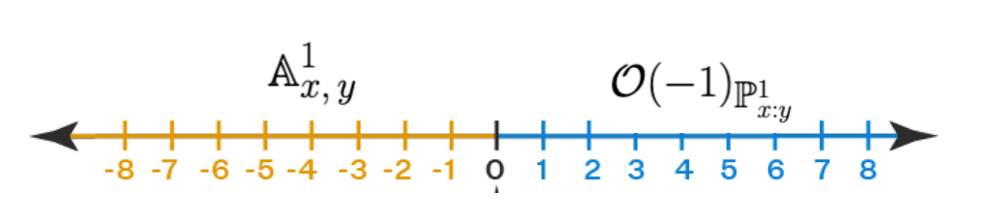
\includegraphics[width=20cm]{diffquotients.png}
    \caption{Secondary fan of GIT problem $\mathbb{C}^3_{(1, \, 1, \, -1 )}$}
  \end{figure} 
\end{example}

\bigskip
\hrule
\end{textblock}

\begin{textblock}{7}(0,9)
  \Head{Mirror Symmetry Conjecture Heuristics}
  \sf
  Mirror symmetry is a series of mysterious relationships between complex and symplectic geometry. Given a \textit{complex geometry} $X$, there exists a mirror \textit{symplectic geometry} $\hat{X}$ such that we have equivalence of categories
  $$
  D^b(X) \cong \text{Fuk}(\hat{X})
  $$
  Actually, we have a whole family of mirrors, each of whom is symplectomorphic to $\hat{X}$, but has a different complex structure. We call the \textcolor{DarkBlue}{\textbf{Stringy Kähler moduli space}} the complex structure moduli space $\mathcal{M}_{CS}$ of the symplectic manifold $\hat{X}$.
  \begin{prop}
    There is a monodromy action of $\pi_1(\mathcal{M}_{CS})$ on $\hat{X}$ via symplectomorphism, and hence an action of $\pi_1(\mathcal{M}_{CS})$ on $\text{Fuk}(\hat{X})$ via autoequivalence.
  \end{prop}
  \begin{center}
  \textcolor{Red}{By mirror symmetry, the action of $\pi_1(\mathcal{M}_{CS})$ carries to an action of $D^b(X)$ via autoequilvance. In the context of Calabi Yau toric GIT, the conjecture is that there is a particular way that $\pi_1(\mathcal{M}_{CS})$ acts,  via spherical twists.}
  \end{center} 
  The program above has been done in certain cases e.g. in \cite{halpern2020combinatorial}.
  \bigskip
  \hrule
  
  \end{textblock}

%----------------------------------------------------------------------%
%           Second column.                                             %
%----------------------------------------------------------------------%
\begin{textblock}{7}(8,2.4)
\Head{Calabi-Yau Toric GIT}
\sf
\begin{defn}
  A GIT problem $(\mathbb{C}^*)^r$ acting on $\mathbb{C}^n$ is \textcolor{DarkBlue}{\textbf{Calabi-Yau}} if the rows of the weight matrix $Q$ add up to 0.
\end{defn}
Suppose $X$ and $Y$ are two GIT quotients. Via wall-crossing you can find a semi-orthogonal decomposition $D^b(X) \cong\langle D^b(Y), \mathcal{C} \rangle$ \cite{derivedgit}. In the Calabi-Yau setting $D^b(X) \cong D^b(Y)$ for any quotients. 
\vspace*{0.7cm} 
\\
Let $A = (a_{ij}) \in M_{(n-r)\times n}(\mathbb{Z})$ be the cokernel of $Q$. Using the CY condition we choose the first row of $A$ to be 1's. The column vectors in $\mathbb{Z}^{n-r}$, called \textcolor{DarkBlue}{\textbf{rays}}, and span a $(n-r-1)$ dimensional polytope $\mathcal{P}(A)$, called the \textcolor{DarkBlue}{\textbf{Primary Polytope}}. Triangulations of $\mathcal{P}(A)$ give us the toric fans for our GIT quotients \cite[Section 4]{coates2018crepant}.
\vspace*{0.7cm} 
\\
The mirror family is a family of Landau Ginsburg Models \cite{cox1999mirror} $\left( (C^*)^{n-r}, W_{\underline{\textbf{a}}} \right)$ where $W_{\underline{\textbf{a}}} : (\mathbb{C}^*)^{n-r} \to \mathbb{C}$:
\begin{align*}
  W_{\underline{\textbf{a}}} \left(X_1, \dots, X_{n-r}\right)  \:= \:&\text{polynomial with coefficients \underline{\textbf{a}} in variables $X_1$}, \\
  &\text{where the powers are given by the entries of } A = (a_{ij}).
\end{align*}
The mirror symmetry statement here says for any GIT quotient $X$,
$D^b(X) \cong FS\left( (C^*)^{n-r}, W_{\underline{\textbf{a}}} \right)$,
where $FS$ is for Fukaya-Seidel category \cite{seidelfukaya}.
\vspace*{0.7cm} 
\\
 $\textbf{a}$ parametrises our mirror family and we have
 $$
\mathcal{M}_{CS} = \left(  (\mathbb{C}^*)^n \backslash \Delta_A \right)/ A \cong (\mathbb{C}^*)^r \backslash \nabla_A
$$
 where the hypersurface $\Delta_A \subset (\mathbb{C}^*)^n$ is called the \textcolor{DarkBlue}{\textbf{$A$-discriminant}} \cite{gelfand1994discriminants}.
\begin{example}
  Suppose $A = (2 \: 1 \: 0)$. Then $W_{a, b, c} (X)= a X^2 + bX +c$. Then $\Delta_A = \{ b^2 = 4ac\} \subset (\mathbb{C}^*)^3$, and using $A$ to scale out $b$, we get $\left(  (\mathbb{C}^*)^3 \backslash \Delta_A \right)/ A \cong \left( (\mathbb{C}^*)^2 \right) \backslash \{ ac =1/4 \}$.
\end{example}
The main observation now is that the discriminant locus arises as the union of components:
$$
\Delta_A = \bigcup_{\Gamma \, \text{min face}} \Delta_\Gamma
$$
The components correspond to \textbf{\textcolor{DarkBlue}{minimal faces}} of $\mathcal{P}(A)$, that is faces whose rays are \textbf{linearly dependent}. \\
$\Gamma$ corresponds to a 'sub GIT problems' $Q_\Gamma$ with non-trivial \textbf{\textcolor{DarkBlue}}{minimal GIT quotients} $Z_{\Gamma}$, where by minimal GIT quotient we mean a GIT quotient that cannot be decomposed further by the wall-crossing. There are spherical functors $F_\Gamma: D^b(Z_\Gamma) \to D^b(X)$ \cite{addington2011new}, where by spherical we mean that the twist
\begin{center}
\begin{tikzcd}
  T_{F_{\Gamma}} = C ( \: FR  \arrow[r,"\text{counit}"] & I_{D^b(X) } \: )
\end{tikzcd}
\end{center}
is an autoequivalence of $D^b(X)$, where $R_\Gamma : D^b(X) \to D^b(Z_\Gamma)$ is the right adjoint.
\textcolor{Red}{
  \begin{center}
  Meridians of the $\Delta_\Gamma$ in $\pi_1(\mathcal{M}_{CS})$ acts on $D^b(X)$ via the spherical twists $T_{F_\Gamma}$.
  \end{center}
}
\hrule
\end{textblock}



\begin{textblock}{7}(8,10.3)
  \Head{Toric Calabi Yau 3-folds of Picard Rank 2}
  
  \sf

  \begin{figure}
    \centering
    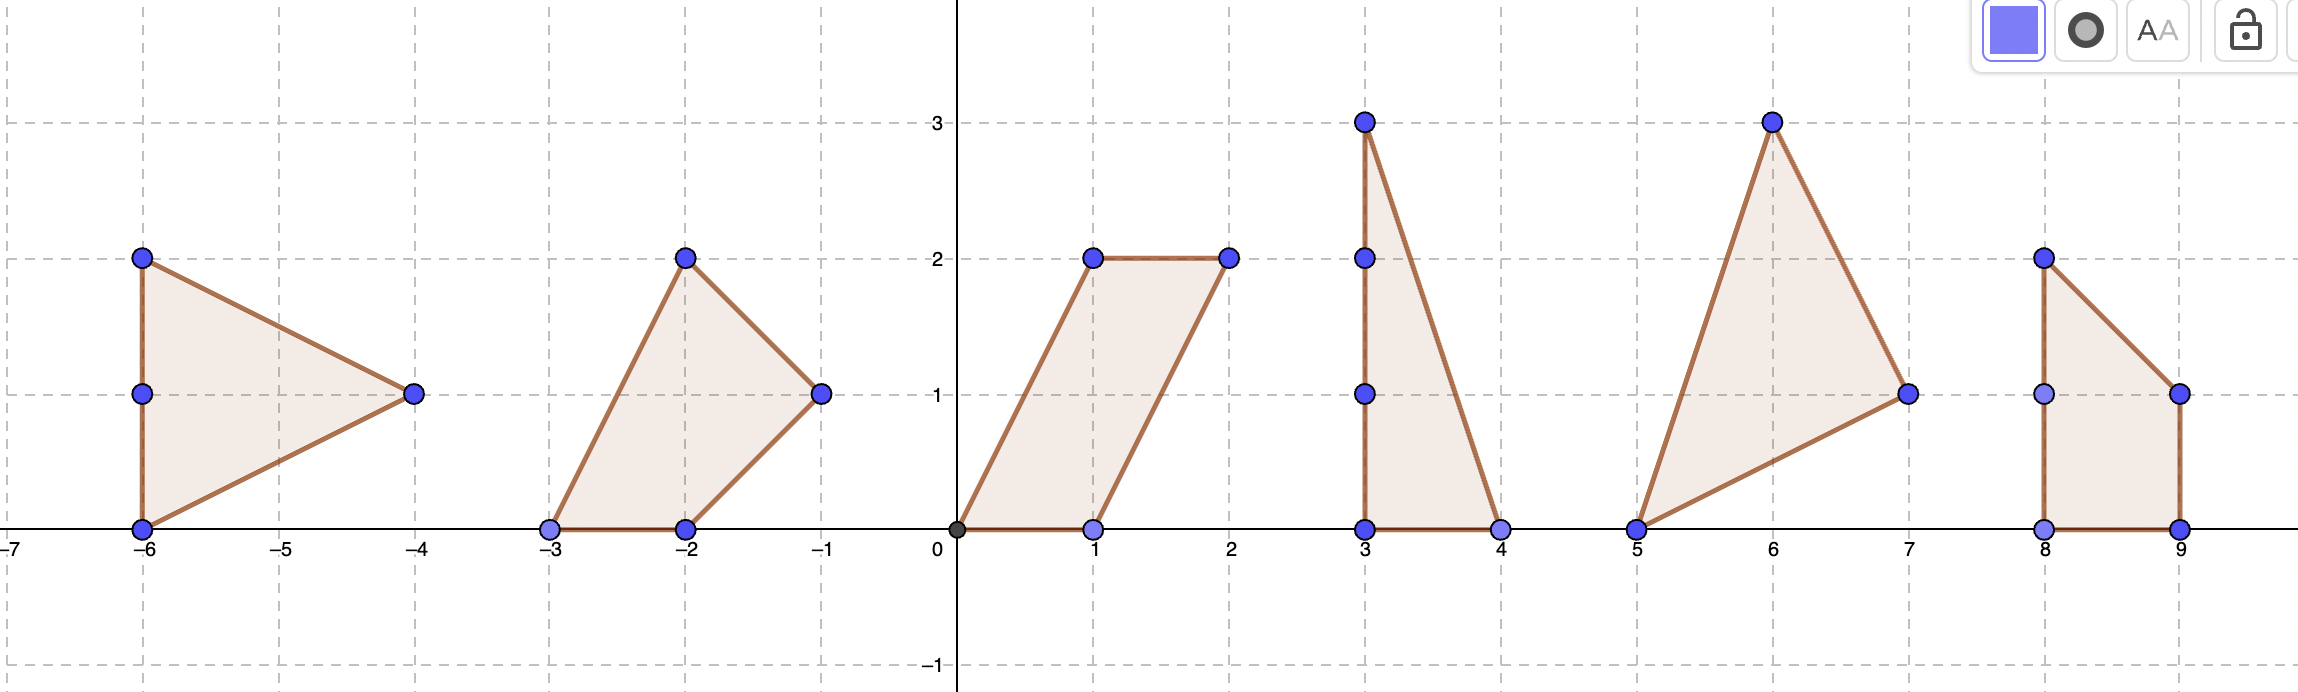
\includegraphics[width=25cm]{3foldsofpicardrank2.png}
    \caption{All the primary polytopes of Toric Calabi Yau 3-folds of Picard Rank 2}
  \end{figure} 
  
  
  \bigskip
  \hrule
  
\end{textblock}


%----------------------------------------------------------------------%
%           Third column.                                              %
%----------------------------------------------------------------------%
\begin{textblock}{7}(16,2.4)

\Head{Rank 2 Example}
\sf
Consider GIT problem
\begin{align*}
Q = \begin{pmatrix}
  -1 & 2 \\
  2 & 0 \\
  -1 & 0 \\
  0 & -1 \\
  0 & -1
\end{pmatrix}
\begin{matrix}
  a \\
  b\\
  c\\
  d\\
  e
\end{matrix}
\hspace*{4cm}
A^T = &\begin{pmatrix}
 1 & 0 & 0 \\
 1 & 1 & 0 \\
 1 & 2 & 0 \\
 1 & 0 & 1 \\
 1 & 0 & -1
\end{pmatrix}
\begin{matrix}
  a \\
  b\\
  c\\
  d\\
  e
\end{matrix}
\end{align*}
We have $$\mathcal{M}_{CS} \cong (\mathbb{C}^{*})^2_{a,b}\backslash \left(\nabla_{\Gamma_0} \cup \nabla_{\Gamma_1} \right) $$
where we can compute
$
\nabla_{\Gamma_0} = \{(b^2-a)^2 = 4\}$ and $\nabla_{\Gamma_1} = \{ a^2 = 4\}.
$
The 'sub GIT problems' $Q_{\Gamma_0}$ and $Q_{\Gamma_1}$, they have minimal GIT quotients $Z_{\Gamma_0} = \text{pt}$ and $Z_{\Gamma_1}= \mathbb{A}^1$, and spherical functors $F_{\Gamma_0} \mathcal{O}_{\text{pt}} = \mathcal{O}_{0} \in D^b(\left[ \mathbb{A}^3 / \mathbb{Z}_4 \right])$ and $F_{\Gamma_0} = i_{*} \pi^{*}$:
\begin{center}
\begin{tikzcd}
  \left[ \mathbb{A}^1_c / \mathbb{Z}_4\right] \arrow[d,"\pi"] \arrow[r, "i"] & \left[\mathbb{A}^3_{c,d,e} / \mathbb{Z}_4 \right] \\
  \mathbb{A}^1_c &
\end{tikzcd}
\end{center}

\begin{figure}
  \centering
  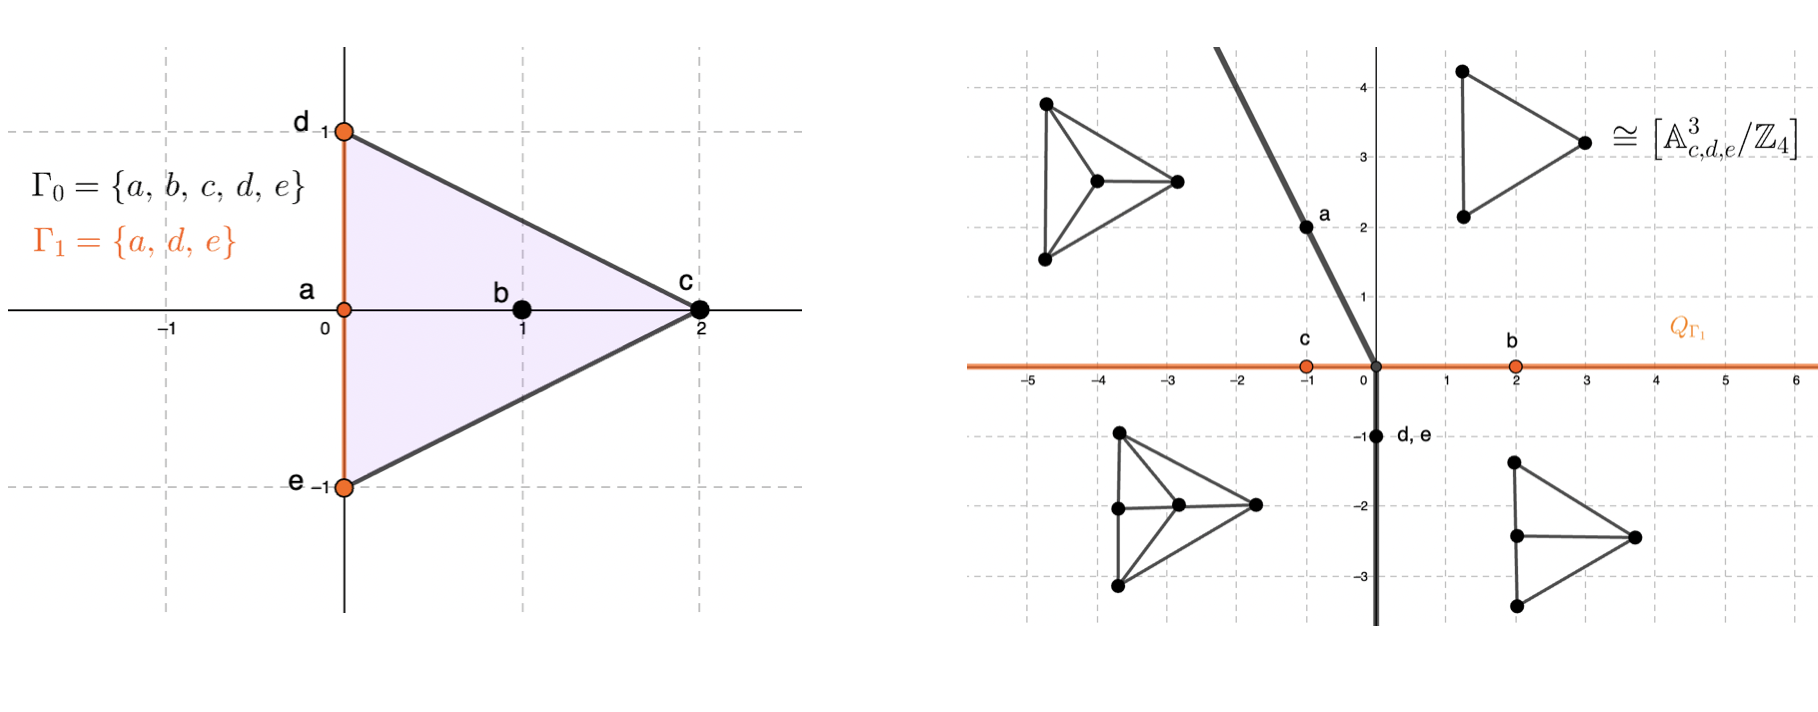
\includegraphics[width=30cm]{rank2.png}
  \caption{Left: The primary polygon $\mathcal{P}(A)$, Right: The secondary fan}
\end{figure}

\begin{lemma}[M. Barbieri 2023]
  The spherical twists $T_{F_{\Gamma_0}}$ and $T_{F_{\Gamma_1}}$ satisfy the relations of a meridian $\mu_{0}$ of $\nabla_{\Gamma_0}$ and a merdian $\mu_{1}$ of $\nabla_{\Gamma_1}$ in $\pi_1(\mathcal{M}_{CS})$.
\end{lemma}

\hrule
\end{textblock}

\begin{textblock}{7}(16, 8.5)
\sf
\bibliographystyle{abbrv}
\bibliography{mybib.bib}
\vspace*{4mm} % Sometimes you will have to fudge the final spacing.

\hrule
\end{textblock}

%----------------------------------------------------------------------%
%            Construction lines                                        %

%\begin{textblock}{23}(0,2)\rule{\textwidth}{0.1mm}\end{textblock}
% Shows where the bottom of the header bar should fall.

%\begin{textblock}{23}(0,2.4)\rule{\textwidth}{0.1mm}\end{textblock}
% Shows where the top of each column should start.

%\begin{textblock}{23}(0,12)\rule{\textwidth}{0.1mm}\end{textblock}
% Shows where the bottom of the lowest block in each column should end

%\begin{textblock}{1.5}(6,4.12)\rule{\textwidth}{0.1mm}\end{textblock}
%\begin{textblock}{1.5}(6,4.52)\rule{\textwidth}{0.1mm}\end{textblock}
% Used to find the base of the first block and thus the top of the second.

%\begin{textblock}{1.5}(14,4.85)\rule{\textwidth}{0.1mm}\end{textblock}
%\begin{textblock}{1.5}(14,5.25)\rule{\textwidth}{0.1mm}\end{textblock}
% Same purpose but in the second column.

%\begin{textblock}{1.5}(15,6.05)\rule{\textwidth}{0.1mm}\end{textblock}
%\begin{textblock}{1.5}(15,6.45)\rule{\textwidth}{0.1mm}\end{textblock}
% Same purpose but in the third column.

\end{document}
